%Stanford, August 14, 2016
\documentclass[12pt,compress,xcolor={usenames,dvipsnames}]{beamer} %slides and notes
\usepackage{amsmath,datetime,xmpmulti,mathtools,bbm,array,booktabs,alltt,xspace,mathabx,pifont,tikz,calc,colortbl,stmaryrd,graphicx}
\usepackage[usenames]{xcolor}
\usepackage[tikz]{mdframed}
\usepackage[author-year]{amsrefs}
\usepackage{newpxtext}
\usepackage[euler-digits,euler-hat-accent]{eulervm}
\usetikzlibrary{arrows}
\usepackage{cleveref}
\usetheme{FJHSlimNoFoot}

\definecolor{ltred}{rgb}{1,0.75,0.75}

\setlength{\parskip}{2ex}
\setlength{\arraycolsep}{0.5ex}

\makeatletter
\newcommand{\vast}{\bBigg@{3}}
\newcommand{\Vast}{\bBigg@{5}}
\makeatother


\mdfdefinestyle{redshade}{%
	leftmargin=0 pt,
	rightmargin = 0pt,
	innerleftmargin = 1ex,
	innerrightmargin = 1ex,
	skipabove = 0 pt,
	skipbelow = 0 pt,
	backgroundcolor=red!20,
	linecolor=red!20,
	roundcorner=5pt}

\title[]{\vspace{3ex}Local Adaption for Univariate Function Approximation and Minimization with Guarantees}
\author[]{Sou-Cheng Choi, Yuhan Ding, Fred J. Hickernell \& Xin Tong }
\institute{%Department of Applied Mathematics,  Illinois Institute of Technology \\
\href{mailto:hickernell@iit.edu}{\url{hickernell@iit.edu}} \quad
\href{http://mypages.iit.edu/~hickernell}{\url{mypages.iit.edu/~hickernell}}}
\thanksnote{Thanks to the IBC 2016 organizers, the GAIL team, and friends\\
	Supported by NSF-DMS-1522687\\[1ex] Happy Birthday Henryk!}
%\date[]{MCQMC \textbullet\ August 14, 2016}

%Title:  Guaranteed Fixed-Width Confidence Intervals for Monte Carlo and Quasi-Monte Carlo Simulation

%Existing adaptive algorithms for function approximation and minimization---such as the Chebfun toolbox [4] and \texttt{fminbnd} in MATLAB [5]---lack theoretical guarantees.  Our new locally adaptive algorithms are guaranteed to provide answers that satisfy a user-specified absolute error tolerance for a cone of non-spiky functions in $W^{2,\infty}$.  These algorithms automatically determine where to sample the function---sampling more densely where needed.  The computational cost to approximate a function with $L^{\infty}$ error no greater than $\varepsilon$ is $\mathcal{O}\Bigl(\sqrt{\lVert f'' \rVert_{\frac 12}/\varepsilon}\Bigr)$, which is the same order as that of the best function approximation algorithm for this cone of functions. This cost may be substantially less than the $\mathcal{O}\Bigl(\sqrt{\lVert f'' \rVert_{\infty}/\varepsilon}\Bigr)$ cost typical of non-adaptive algorithms.  The computational cost of the new minimization algorithm is asymptotically no worse than that for function approximation.  The cost of minimization can be much smaller if the function being minimized is significantly larger than its minimum value over much of its domain.  This work extends the ideas of [2, 3, 6]. Our new algorithms have been implemented in a software library [1].  Numerical examples are presented to illustrate the advantages of these new algorithms.


\input FJHDef.tex
\renewcommand{\mSigma}{\Sigma}
\newcommand{\smallcite}[1]{{\small\cite{#1}}}
\newcommand{\smallocite}[1]{{\small\ocite{#1}}}
\newcommand{\smallcites}[1]{{\small\cites{#1}}}
\newcommand{\tol}{\text{tol}}
\newcommand{\Phnu}{\Prob_{\hnu}}
\DeclareMathOperator{\init}{init}
\DeclareMathOperator{\hugetext}{huge}
\DeclareMathOperator{\oerr}{\overline{err}}
\DeclareMathOperator{\herr}{\widehat{e}}
\DeclareMathOperator{\cubMC}{cubMC}
\DeclareMathOperator{\qse}{qse}
\DeclareMathOperator{\integ}{int}
\DeclareMathOperator{\trap}{trap}
\DeclareMathOperator{\size}{size}
\DeclareMathOperator{\app}{id}
\DeclareMathOperator{\err}{err}
\DeclareMathOperator{\MSE}{MSE}
\DeclareMathOperator{\RMSE}{RMSE}
\DeclareMathOperator{\PProb}{\mathbb{P}}
\DeclareMathOperator{\walsh}{walsh}
\newcommand{\happ}{\widehat{\app}}
\newcommand{\hinteg}{\widehat{\integ}}
\newcommand{\cube}{[0,1)^d}
\newcommand{\desall}{\{\vz_i\}}
\newcommand{\desn}{\{\vz_i\}_{i=0}^{n-1}}
\def\newblock{\hskip .11em plus .33em minus .07em}
\newcommand{\wcS}{\widecheck{S}}
\newcommand{\wcomega}{\widecheck{\omega}}
\newcommand{\HickernellFJ}{H.} %To give my name to the bibliography
\newcommand{\abstol}{\varepsilon}
\newcommand{\reltol}{\varepsilon_{\text{r}}}
\DeclareMathOperator{\MLE}{MLE}
\DeclareMathOperator{\algn}{ALN}
\DeclareMathOperator{\disc}{DSC}
\DeclareMathOperator{\Var}{VAR}
\DeclareMathOperator{\RMS}{RMS}
\DeclareMathOperator{\GP}{\cg\cp}
\newcommand{\Dt}{\text{D}}
\newcommand{\Rn}{\text{R}}
\newcommand{\Ba}{\text{B}}
\newcommand{\tmC}{\widetilde{\mC}}
\newcommand{\tvC}{\widetilde{\vC}}
\newcommand{\vC}{\boldsymbol{C}}
\newcommand{\hvtheta}{\hat{\vtheta}}
\newcommand{\hs}{\hat{s}}
\newcommand{\fn}{\mathfrak{n}}

\newcommand{\redroundmathbox}[1]{\parbox{\widthof{$#1$\hspace{1em}}}
	{\begin{mdframed}[style=redshade]\centering $#1$ \end{mdframed}}}
\newcommand{\setbeameruncoveredtransp}{\setbeamercovered{transparent=10}}
\newcommand{\shadegraph}[1]{\tikz\node[opacity=0.25, inner sep=0, outer sep=0]{#1};}
\newcommand{\sleepPict}{\href{http://www.preapps.com/blog/wp-content/uploads/2015/09/Valuable-Sleep.jpg}{\includegraphics[width = 3cm]{ProgramsImages/Valuable-Sleep.jpg}}}
\newcommand{\financePict}{\href{http://i2.cdn.turner.com/money/dam/assets/130611131918-chicago-board-options-exchange-1024x576.jpg}{\includegraphics[width = 3cm]{ProgramsImages/130611131918-chicago-board-options-exchange-1024x576.jpg}}}
\newcommand{\GaussPict}{\href{http://www.mathworks.com/matlabcentral/answers/uploaded_files/26298/Plotting\%20a\%203d\%20gaussian\%20function\%20using\%20surf\%20-\%202015\%2002\%2027.png}{\includegraphics[width = 3cm]{ProgramsImages/Plotting_gaussian.png}}}

\newcommand{\medcone}{\parbox{1.2cm}{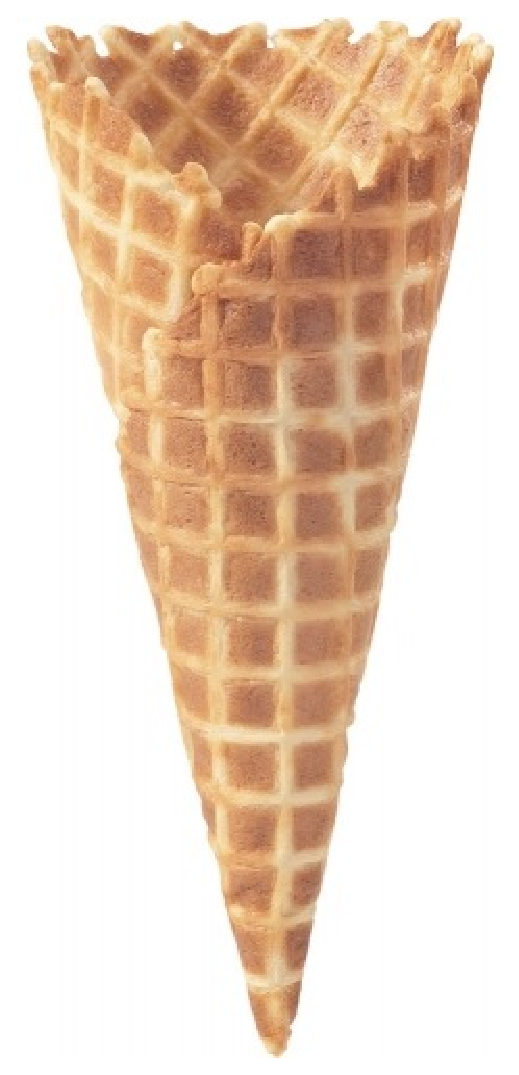
\includegraphics[width=0.55cm,angle=270]{ProgramsImages/MediumWaffleCone.eps}}\xspace}

\newcommand{\smallcone}{\parbox{0.65cm}{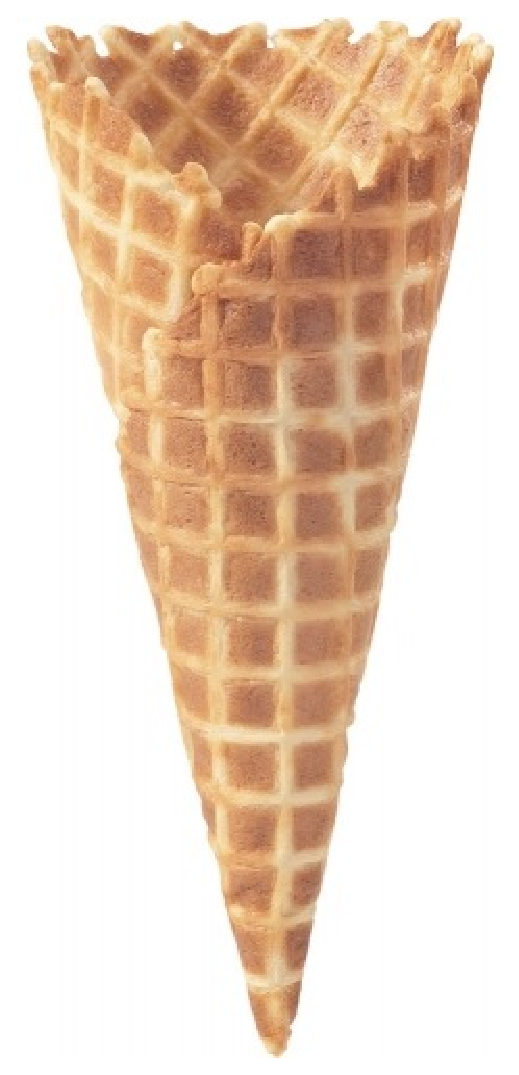
\includegraphics[width=0.3cm,angle=270]{ProgramsImages/MediumWaffleCone.eps}}\xspace}

\newcommand{\lecone}{\smallcone\hspace*{-0.3cm}\mathclap{\le}\hspace*{0.35cm}}

\definecolor{MATLABBlue}{rgb}{0, 0.447, 0.741}
\definecolor{MATLABOrange}{rgb}{0.85,  0.325, 0.098}
\definecolor{MATLABPurple}{rgb}{0.494,  0.184, 0.556}
\definecolor{MATLABGreen}{rgb}{0.466,  0.674, 0.188}

\newcommand{\northeaststuff}[3]{
	\begin{tikzpicture}[remember picture, overlay]
	\node [shift={(-#1 cm,-#2 cm)}]  at (current page.north east){#3};
	\end{tikzpicture}}




\begin{document}
\tikzstyle{every picture}+=[remember picture]
\everymath{\displaystyle}

\frame{\titlepage}

\section{Problem}

\begin{frame}<1>[label = Goal, fragile]
	\frametitle{\only<1>{Done Already}\only<2>{Goal}}
	\northeaststuff{3.7}{2.2}{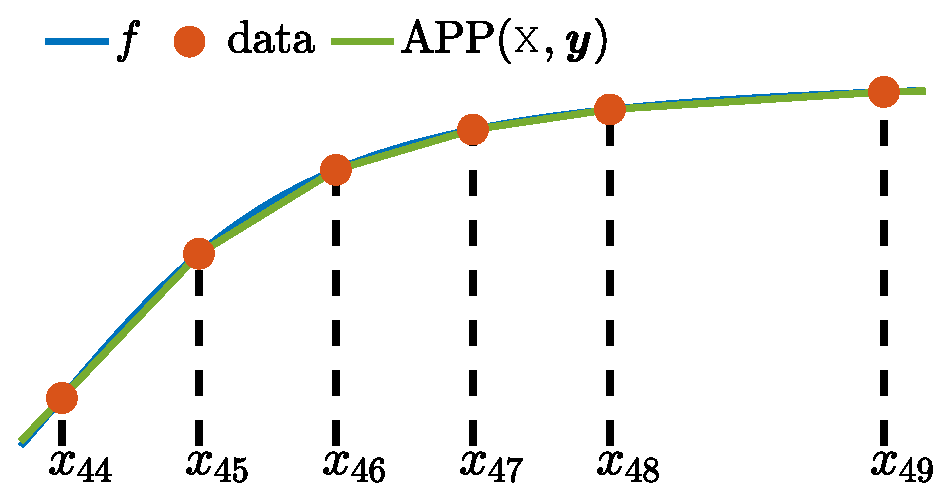
\includegraphics[width=7cm]{ProgramsImages/LinearSpline.eps}}
	
	\vspace{-1ex}
	
Given 

	\vspace{-3ex}
	\begin{itemize}
		\item \alert{function}, $f:[a,b] \to \reals$, 
		\item \alert{error tolerance}, $\varepsilon$, and 
		\item<only@1> \alert{ball} $\cb = \{f \in \cw^{2,\infty}: \norm{f''} \le \alert{\sigma} \}$ of radius \alert{$\sigma$}
		\item<only@2> nonconvex \alert{cone} $\cc \subset \cw^{2,\infty}$ defined by constants $n_{\init}$ and $\fC_0$
	\end{itemize}
		\vspace{-3ex}
	\only<1>{one may \alert{nonadaptively}}\only<2>{we \alert{adaptively}} construct a linear spline, $S(f,x_{0:n})$ with \only<1>{$x_i = a + i(b-a)/n,\ i=0:n$}\only<2>{$a = x_0 <x_1 < \cdots < x_n = b$}, satisfying $\forall f \in \only<1>{\cb}\only<2>{\cc}$ \only<2>{\cite{ChoEtal17a}}
	\begin{gather*}
	\norm{f - S(f,x_{0:n})} \overset{\text{\alert{always}}}{\le}  \max_{i=1:n}\frac{1}{8}(x_{i}-x_{i-1})^2\norm[{[x_{i-1},x_i]}]{f''} \only<1>{ \le \frac{(b-a)^2\alert{\sigma}}{8 n^2}} \overset{\text{\alert{goal}}}{\le} \varepsilon  \\
	\only<1>{\sqrt{\frac{\alert{\sigma}}{\varepsilon}} \asymp \comp(\varepsilon,\alert{\sigma},\cb) \le \cost(S,\varepsilon, \alert{\sigma}, \cb) = n+1 \\[-1ex] \hspace{30ex} = \left \lceil (b-a)\sqrt{\frac{\alert{\sigma}}{8\varepsilon}} \, \right \rceil + 1}
	\only<2>{\sqrt{\frac{\norm[\alert{\frac12}]{f''}}{\varepsilon}} \asymp \comp(\varepsilon,f, \cc) \le \cost(S, \varepsilon, f, \cc) = n+1 \asymp \sqrt{\frac{\norm[\alert{\frac12}]{f''}}{\varepsilon}} \\
		\comp\Bigl(\varepsilon,\sigma, \Bigl\{f \in \cw^{2,\infty}: \norm[\alert{\frac12}]{f''} \le \sigma\Bigr\}\Bigr) = \infty }
	\end{gather*}
	
	
\end{frame}

\begin{frame}
	\frametitle{State of the Art}
	
	\vspace{-3ex}
	
	\begin{itemize}
		\item Algorithms with \alert{theoretical justification} require bounds on the (semi-)norms of functions---impractical
		
		\item Popular adaptive algorithms have no sufficient conditions for success, e.g., \alert{Chebfun} \cite{TrefEtal16b} uses Chebyshev polynomials to approximate, integrate, optimize, etc.\ functions 
		
		\item Successful optimization algorithms require the input function to be \alert{convex}
		
		\item Guaranteed algorithms exist based on \alert{interval arithmetic} \cites{Rum99a, Rum10a}, but we do not want to follow that model
		
		\item \emph{We show that \alert{adaption does not help} for linear problems for the worst case setting [for a balanced, convex set of input functions] \ldots } \alert{\cite{Woz88a}}
		
    	\item \ocite{PlaEtal08a} have approximation algorithms for functions with \alert{singularities}
		
		
	\end{itemize}
\end{frame}

\againframe<2>{Goal}

\begin{frame}
	\frametitle{Bounding $\norm[{[\alpha,\gamma]}]{f''}$}
		\northeaststuff{3.7}{2.2}{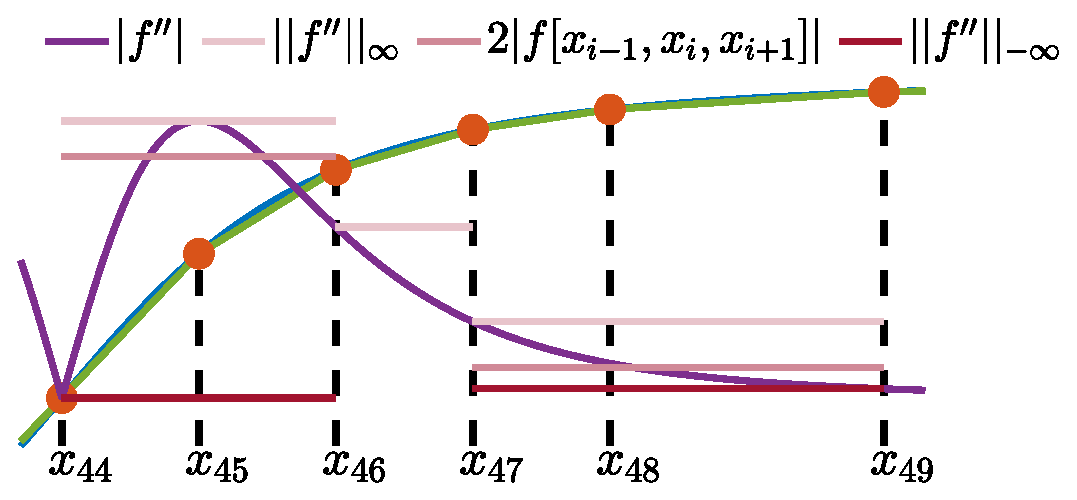
\includegraphics[width=7cm]{ProgramsImages/LinearSplineSecDeriv.eps}}
		
		\begin{multline*}
		\inf_{\alpha \le \xi < \zeta \le \gamma} \abs{\frac{f'(\zeta) - f'(\xi)}{\zeta - \xi}} = \norm[{-\infty, [\alpha,\gamma]}]{f''} \\
		\le 2\abs{f[\alpha,\beta,\gamma]} = 2 \abs{\frac{\frac{f(\gamma) - f(\beta)}{\gamma - \beta} - \frac{f(\beta) - f(\alpha)}{\beta - \alpha}}{\gamma - \alpha}} \alert{\leftarrow \text{ data}}\\
		\le \norm[{[\alpha,\gamma]}]{f''} = \sup_{\alpha \le \xi < \zeta \le \gamma} \abs{\frac{f'(\zeta) - f'(\xi)}{\zeta - \xi}}
		\end{multline*}
		\vspace{-4.5ex}
		
		\uncover<2>{We construct our \alert{adaptive} spline algorithm for functions in 
		
		\vspace{-6.2ex}
		\begin{multline*}
		\cc \ \text{``}\!\!=\!\!\text{''} \ \Bigl\{f : \norm[{[\alpha,\gamma]}]{f''} \le \max \bigl (\fC(h_{-}) \norm[{-\infty,[\gamma - h_-, \alpha]}]{f''}, \\[-1ex] \fC(h_{+})\norm[{-\infty,[\gamma,\alpha + h_+ ]}]{f''} \bigr), \ 
		\gamma - \alpha \le h_{\pm} < \fh\Bigr\}
		\end{multline*}}
\end{frame}

\begin{frame}
	\frametitle{Cone of Reasonable Functions, $\cc$}
	\northeaststuff{3.7}{3}{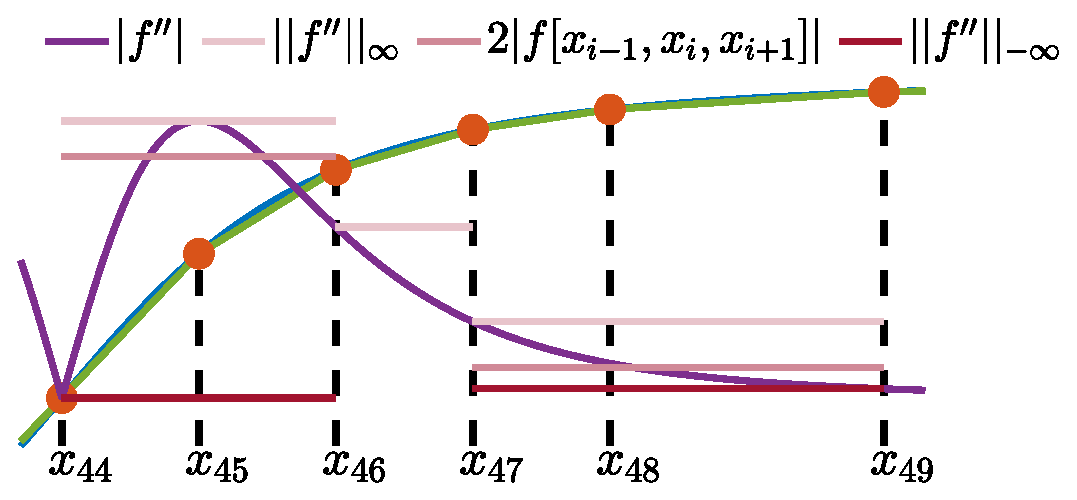
\includegraphics[width=7cm]{ProgramsImages/LinearSplineSecDeriv.eps}}

\vspace{-10ex}

\parbox{4.2cm}{
	\begin{align*}
	 \norm[{-\infty, [\alpha,\gamma]}]{f''}
	& \le 2\abs{f[\alpha,\beta,\gamma]} \\ & \le \norm[{[\alpha,\gamma]}]{f''}
	\end{align*}
	
	\vspace{-1.5ex}
	Given $n_{\init} \ge 4$, $\fC_0 \ge 1$: 
	
	\vspace{-3.5ex}
	
	\begin{gather*}
	\fh  = \left \lceil \frac{3(b-a)}{n_{\init}-1} \right \rceil \\ \fC(h) = \frac{\fC_0 \fh}{\fh - h}
	\end{gather*}}

\vspace{-4ex}

We construct our \alert{adaptive} spline algorithm for functions in 
	
	\vspace{-5.5ex}	
		\begin{gather*}
		\cc =  \Bigl\{f : \norm[{[\alpha,\gamma]}]{f''} \le \max \bigl (B_{\pm}(f'',\alpha,\gamma,h_{\pm})  \bigr), \ \gamma - \alpha \le h_{\pm} < \fh\Bigr\} \\[-1ex]
		B_{-}(f'',\alpha,\gamma,h_-) = \begin{cases} \fC(h_{-}) \norm[{-\infty,[\gamma - h_-, \alpha]}]{f''}, & a \le \gamma - h_- \\
		0, & \text{otherwise} \end{cases} \\
		B_{+}(f'',\alpha,\gamma,h_+) = \begin{cases} \fC(h_{+})\norm[{-\infty,[\gamma,\alpha + h_+ ]}]{f''}, & \alpha + h_+ \le b \\
		0, & \text{otherwise} \end{cases} \\
		\end{gather*}
\end{frame}

\section{Approximation Algorithm}
\begin{frame}
	\frametitle{Local Spline Error Bounds for $\cc$}
	\northeaststuff{3.7}{3}{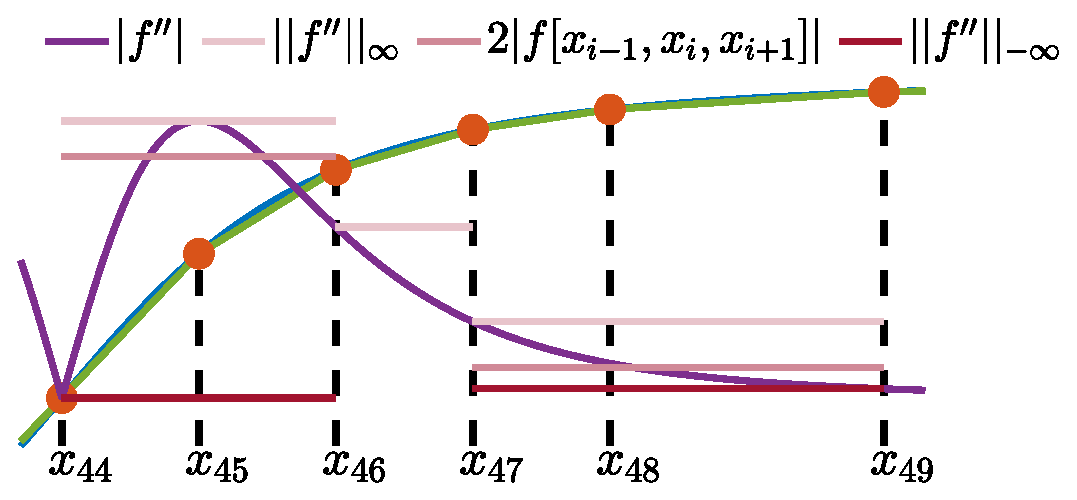
\includegraphics[width=7cm]{ProgramsImages/LinearSplineSecDeriv.eps}}
	
	\vspace{-8ex}
	
	\parbox{4.2cm}{
		Use divided differences to construct spline error bounds
		\begin{multline*}
		\norm[{[x_{i-1},x_i]}]{f - S(f,x_{0:n})} \\ \le \max_{\pm} \oerr_{i,\pm}(f)
		\end{multline*}
		}

	
	\vspace{-4ex}
		
	where
	
	\vspace{-4ex}	
	\begin{gather*}
	\oerr_{i,-}(f) = \begin{cases} \frac 14 (x_i-x_{i-1})^2\fC(x_i - x_{i-3}) \abs{f[x_{i-3},x_{i-2},x_{i-1}]}, & i \ge 3\\
	0, & \text{otherwise} \end{cases} \\
	\oerr_{i,+}(f) = \begin{cases} \frac 14 (x_i-x_{i-1})^2\fC(x_{i+2} - x_{i-1}) \abs{f[x_{i},x_{i+1},x_{i+2}]}, & i \le n-2 \\
	0, & \text{otherwise} \end{cases} \\
	\end{gather*}
\end{frame}

\begin{frame}
	\frametitle{Approximation Algorithm}
	\northeaststuff{3.7}{3}{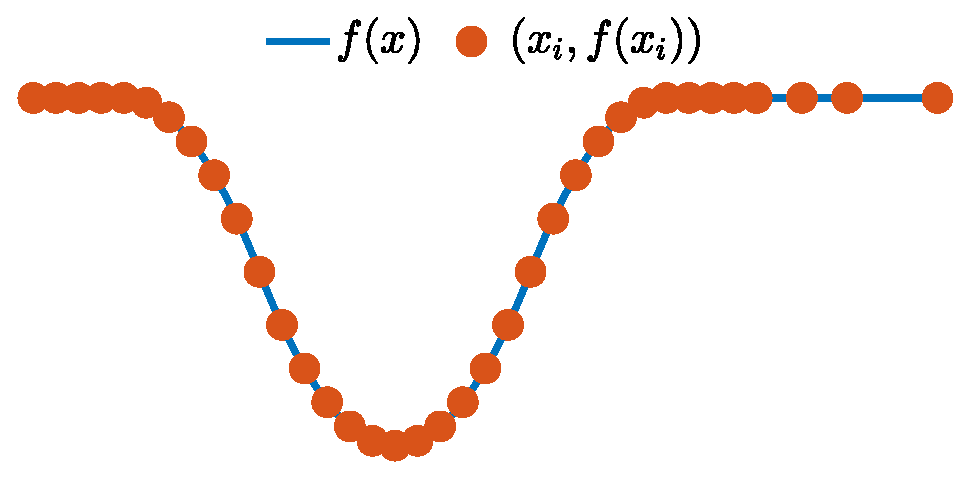
\includegraphics[width=7cm]{ProgramsImages/sampling-funappxg.eps}}
	
	\vspace{-8ex}
	
		\parbox{4.2cm}{
			Given $n_{\init} \ge 4$, $\fC_0 \ge 1$: 
			
			\vspace{-3.5ex}
			
			\begin{gather*}
			\fh  = \left \lceil \frac{3(b-a)}{n_{\init}-1} \right \rceil \\ 
			\fC(h) = \frac{\fC_0 \fh}{\fh - h} \\
			n = n_{\init} \\
			x_i = a + i(b-a)/n
			\end{gather*}
			}
		
	
	\vspace{-4ex}
	
\begin{description}
	\item[Step 1.] Compute data based $\oerr_{i\pm}(f)$ for $i = 1, \ldots, n$.
	\item[Step 2.] Construct $\ci$, the index set of subintervals that might be split:
	\begin{equation*}
	\ci = \bigl\{i \in 1\! :\! n \ : \ \oerr_{i\pm j,\mp}(f) > \varepsilon, \ j = 0, 1, 2\}
	\end{equation*}
	\item[Step 3.]  If $\ci = \emptyset$, return $S(f,x_{0:n})$ as the approximation satisfying the error tolerance.  Otherwise split those intervals in $\ci$ with largest width and go to Step 1. 
\end{description}
	
\end{frame}

\begin{frame}
	\frametitle{Computational Cost of Function Approximation}
	\vspace{-6.5ex}
	\begin{align*}
	h_{\init}  &= \frac{b-a}{n_{\init}},  \quad  h_{\init} 2^{-\ell(x)} = \text{final width of subinterval containing } x \\
	 I_{x}& =\text{interval containing $x$ with width } 10 \cdot h_{\init} 2^{-\ell(x)} \\
\end{align*}
\vspace{-6ex}
\begin{align*}
	\cost(S,f,\varepsilon,\cc) 
		&= \int_a^b \frac{\dif x}{\text{final width of subinterval containing } \alert{x}} \,  + 1\\
		&= \int_a^b \frac{\dif x}{h_{\init} 2^{-\ell(\alert{x})}} \,  + 1\\
	&\le \int_a^b \sqrt{\frac{\fC\left(6\cdot 2^{-\ell(\alert{x})} h_{\init}\right) \norm[I_{\alert{x}}]{f''} }{2 \abstol}}  \, \dif x + 1\\
	& \sim \sqrt{\frac{\fC_0 \norm[\alert{\frac 12}]{f''}}{2\abstol}}  \quad \text{ as } \varepsilon \to 0 \\
	\comp(\varepsilon,f,\cc) &\ge \sqrt{\frac{(\fC_0-1)  \norm[\frac12]{f''} }{16(\fC_0+1)\varepsilon}} -1 \quad \text{via bump functions}
	\end{align*}
\end{frame}

\section{Function Minimization}
\begin{frame}
	\frametitle{Global Minimization of a Function}
		\vspace{-4ex}
		
		Given 
		
		\vspace{-3ex}
		\begin{itemize}
			\item \alert{function}, $f:[a,b] \to \reals$, 
			\item \alert{error tolerance}, $\varepsilon$, and 
			\item \alert{cone} $\cc \subset \cw^{2,\infty}$ defined by constants $n_{\init}$ and $\fC_0$
		\end{itemize}
		\vspace{-3ex}
		we \alert{adaptively} choose $n$ and points $x_{0:n}$ with $a = x_0 <x_1 < \cdots < x_n = b$, satisfying
		\begin{equation*}
		\min f(x_{0:n}) - \min_{a \le x \le b} f(x)  \overset{\text{\alert{goal}}}{\le} \varepsilon \quad \forall f \in \cc 
		\end{equation*}
	using the fact that
	\begin{align*}
	\min(f(x_{i-1}), f(x_i)) - \min_{x_{i-1} \le x \le x_i} f(x) & \le \frac{1}{8}(x_{i}-x_{i-1})^2\norm[{[x_{i-1},x_i]}]{f''} \\
	& \le \max_{\pm} \oerr_{i,\pm}(f)
	\end{align*}
	The $i^{\text{th}}$ interval and its neighbors are candidates for splitting if 
	\[
	\oerr_{i,\pm}(f) > \varepsilon + \min(f(x_{i-1}), f(x_i)) - \min f(x_{0:n})
	\]
		
\end{frame}

\begin{frame}
	\frametitle{Global Minimization Example}
\centerline{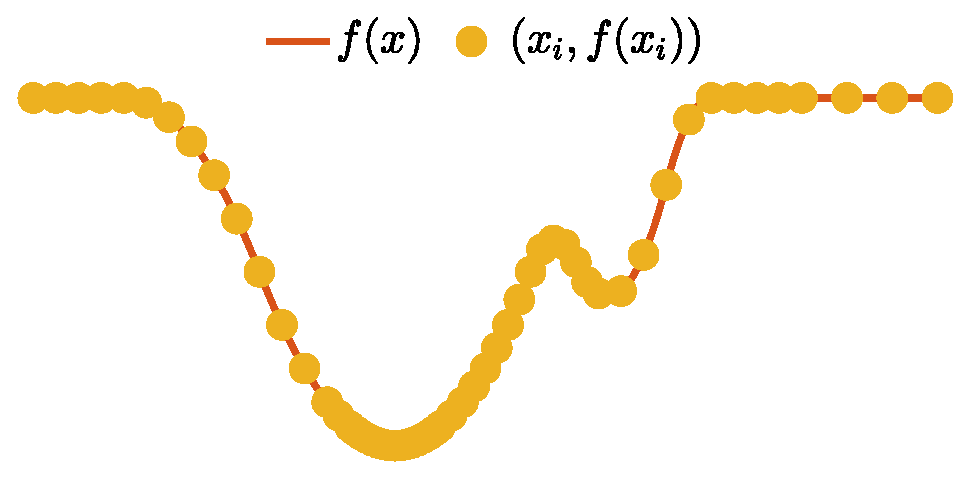
\includegraphics[width = 11.5cm]{ProgramsImages/sampling-funming.eps}}
\end{frame}


\section{Take Home}
\begin{frame}
	\frametitle{Take Home Points }
	\vspace{-2ex}
\begin{itemize}
	\item New \alert{locally} adaptive (non-uniform sampling density)  algorithms for univariate function approximation and global minimization---implemented in GAIL \cite{ChoEtAl15a}
	
	\item Algorithms succeed for \alert{cones} of input functions, continuing the theme of \cites{HicEtal14a,HicEtal14b,Ton14a,Din15a,Jia16a}
	
	\item Computational cost of our function approximation algorithm is $\asymp \sqrt{\norm[\alert{\frac12}]{f''}/\varepsilon}$---asymptotically optimal
	
	\item Need \alert{higher order} algorithms---is their computational cost $\asymp \left(\norm[\frac1r]{f^{(r)}}/\varepsilon\right)^{1/r}$?
	
	%\item Local adaption may be practical for \alert{multidimensional} problems with lower dimension, but would they work in high dimension?
	
	\end{itemize}
	
	\bigskip
	
	\uncover<2->{\centerline{\Large \alert{Think globally, act locally\uncover<3->{---like Henryk}}}}
	
\end{frame}

\begin{frame}[allowframebreaks]\frametitle{References}
	\bibliography{FJH23,FJHown23}
\end{frame}

\end{document}

